\documentclass[../main.tex]{subfiles}

\begin{document}


%
% -----------------------------------------------------------------------------------------------------------------
%


\begin{frame}[t]{Motivation}

\textbf{Motivation}: Tendecy to reconfigurable phased array antennas.

\textbf{Examples}:

\begin{itemize}
    \item Dual-function radar communication (DFRC)
    \item 
\end{itemize}

\textbf{Main reasons}: 
\begin{itemize}
    \item Spectrum congestion problem
    \item Reduced cost, size and weight
\end{itemize}


\end{frame}


%
% ----------------------------------------------------------------------------------------------------------------- 
%



\begin{frame}[t]{Reconfigurable phased antenna arrays. Power amplifier non-linearity}

\textbf{Input}: signals $f_1$ and $f_2$

\textbf{Output}: 
\begin{itemize}
    \item $f_1, f_2$
    \item 2nd harmonics ($2f_1, 2f_2$) and distortion products ($f_2 \pm f_1$)
    \item 3rd order distortion ($2f_1 \pm f_2$, $2f_2 \pm f_1$)
\end{itemize}

\begin{figure}[H]
\begin{adjustbox}{width=0.6\columnwidth}
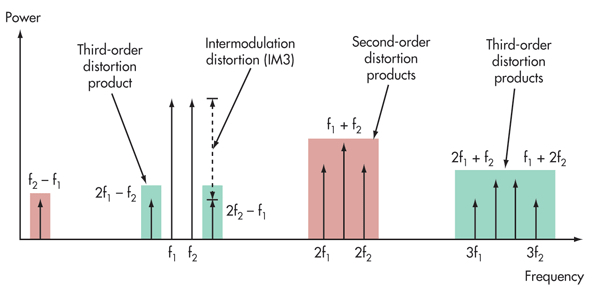
\includegraphics{pics/IMD.jpg}
\end{adjustbox}
\end{figure}


\end{frame}


%
% -----------------------------------------------------------------------------------------------------------------
%

\begin{frame}[t]{Multi-frequency antenna elements allocation}

\begin{figure}[H]
  \centering
  \begin{tikzpicture}
    \draw[thin, color=gray!50] (0, 0) -- (0, 0.5);
    \draw[thin, color=gray!50] (1, 0) -- (1, 0.5);
    \draw[thin, latex'-latex'] (0, 0.5) -- node[above]{$d$} (1, 0.5);

    \draw[thin, -latex', color=gray] (0, 0) -- (-1, 1);
    \coordinate (a1) at (-1, 0);
    \coordinate (b1) at (0, 0);
    \coordinate (c1) at (-1, 1);
    \pic["$\phi_{m}$", draw,<-,>=stealth,angle eccentricity=1.7, angle radius=0.5cm] {angle=c1--b1--a1};
    \draw[thin] (a1) -- (b1);
    \draw[fill] (0,0) circle [radius=0.1] node[below left]{\scriptsize $1$};
    \draw[thin, -latex'] (0, -1) node[below]{$I^{\lambda_k}_1$} -- (0, -0.1);

    \draw[fill] (1,0) circle [radius=0.1] node[below left]{\scriptsize $2$};
    \draw[thin, -latex'] (1, -1) node[below]{$I^{\lambda_k}_2$} -- (1, -0.1);

    \draw[thin, -latex', color=gray] (2, 0) -- (1, 1);
    \draw[fill] (2,0) circle [radius=0.1] node[below left]{\scriptsize $3$};
    \draw[thin, -latex'] (2, -1) node[below]{$I^{\lambda_k}_3$} -- (2, -0.1);

    \draw[draw=black, dotted] (-0.4, -1) rectangle node[below=0.5cm]{$I^{\lambda_k}$} (2.4, -1.7);

    \draw[thin, -latex', color=gray] (3, 0) -- (2, 1);
    \draw[fill] (3,0) circle [radius=0.1] node[below left]{\scriptsize $4$};
    \draw[thin, -latex'] (3, -1) node[below]{$I^{\lambda_{l}}_1$} -- (3, -0.1);

    \draw[dotted, thin](3.5, 0) -- (4.5, 0);

    \draw[thin, -latex', color=gray] (5, 0) -- (4, 1);
    \draw[fill] (5,0) circle [radius=0.1] node[below left]{\scriptsize $N-1$};
    \draw[thin, thin, -latex'] (5, -1) node[below]{$I^{\lambda_{l}}_n$} -- (5, -0.1);
    
    \draw[thin, -latex', color=gray] (6, 0) -- (5, 1);
    \draw[fill] (6,0) circle [radius=0.1] node[below left]{\scriptsize $N$};
    \draw[thin, thin, -latex'] (6, -1) node[below]{$I^{\lambda_{l}}_{n+1}$} -- (6, -0.1);

    \draw[draw=black, dotted] (2.6, -1) rectangle node[below=0.5cm]{$I^{\lambda_l}$} (6.4, -1.7);

  \end{tikzpicture}
\end{figure}

\begin{itemize}
	\item $I^{\lambda_{l}}$ and $I^{\lambda_{k}}$ represent randomly allocated currents with wavelengths $\lambda_l$ and $\lambda_k$ for illustration purposes
	\item $\phi_{m}$ is the beam angle, $d$ is the distance between antenna elements
\end{itemize}

\end{frame}


%
% -----------------------------------------------------------------------------------------------------------------
%

\begin{frame}[t]{Problem formulation}

\textbf{Given:} antenna configuration ($d, N$), reference patterns at different frequencies.

\textbf{Find:} optimal allocation of currents among antenna elements
    
\begin{equation*}
\begin{aligned}
& \minimise_{I^{\lambda_{1\ldots k}}} 
& & \Big\| \mathcal{F}^{\lambda_{1 \ldots k}} I^{\lambda_{1\ldots k}} - b^{\lambda_{1 \ldots k}} \Big\|_2^2 \\
& \st
& & I^{\lambda_i} \odot I^{\lambda_j} = 0, \quad \forall i, j \colon i \ne j \\
\end{aligned}
\end{equation*}

where 
\begin{equation*}
  \mathcal{F}_{\lambda_{1 \ldots k}} = \diag{(\mathcal{F}_{\lambda_1}, \mathcal{F}_{\lambda_2}, \ldots, \mathcal{F}_{\lambda_k})}, \quad \mathcal{F}_{\lambda_{k}} = \Big\{ e^{i \frac{2\pi}{\lambda_k}n d \cos{\phi_m}} \Big\}_{n=0\ldots N, m = 0\ldots M}
\end{equation*}

\textbf{Note}: 
\begin{itemize}
    \item The problem is non-convex, non-linear with a combinatorial constraint, i.e. $(k+1)^N$ solutions should be tested ($k$ - number of frequencies, $N$ - number of elements).
\end{itemize}

\end{frame}


%
% -----------------------------------------------------------------------------------------------------------------
%



\begin{frame}[t]{Results}

For $2$ different currents:

\begin{equation*}
\begin{aligned}
& \minimise_{I^{\lambda_{1\ldots k}}} 
& & \Big\| \mathcal{F}^{\lambda_{1 \ldots k}} I^{\lambda_{1\ldots k}} - b^{\lambda_{1 \ldots k}} \Big\|_2^2 \\
& \st
& & (I^{\lambda_{1\ldots k}})^T B I^{\lambda_{1\ldots k}} = 0 \\
&&& I^{\lambda_{1\ldots k}} \succeq 0 \\
\end{aligned}
\end{equation*}
where $B$ is backward identity matrix, i.e. $\begin{bmatrix} 0 & I \\ I & 0\end{bmatrix}$


Non-trivial lower bound can be obtained:

\begin{equation*}
\begin{aligned}
& \min_{x} 
& & \Big\{\| Ax - b \|_2^2 + \lambda_{min} (A^TA) x^T B x \Big\} \\
& \st
& & x \ge 0 \\
\end{aligned}
\end{equation*}

\end{frame}





%
% -----------------------------------------------------------------------------------------------------------------
%

\begin{frame}[t]{Power pattern. Uncertainty principle}

\begin{equation*}
\Big\| |\mathcal{F}^{\lambda_{1 \ldots k}} I^{\lambda_{1\ldots k}}|^2 - |b^{\lambda_{1 \ldots k}}|^2 \Big\|_2^2 = \sum_{k=1}^K \sum_{m=1}^M \Big\| (I^{\lambda_{k}})^T Q^{\lambda_{k}}_m  I^{\lambda_{k}} - |b^{\lambda_{k}}_m|^2 \Big\|_2^2
\end{equation*}


 
\begin{itemize}
	\item It can be shown that the gradient of the objective function is non-zero everywhere except solution if $\mathcal{N}_{+}(Q_i) = \varnothing, ~\forall i$
	\item Analysis of $\mathcal{N}_{+}(Q_i)$ leads to the following conditions:
	\begin{equation*}
  \frac{d}{\lambda} \neq \frac{k}{N+1} \sec \phi_m , \quad \frac{d}{\lambda} \neq \frac{1}{2N} (1 + 2k) \sec \phi_m, \quad \forall m \in \mathbb{Z}^{\ge 0}, \forall k \in \mathbb{Z}
  \label{antenna_design_condition}
	\end{equation*}
	\item These conditions can be interpreted as an \textbf{uncertainty principle} for antenna design: 
\end{itemize}

\begin{center}
\begin{tcolorbox}
\textit{The finer the spacial resolution of the beam is the more values of $\frac{d}{\lambda}$ should be avoided in favour of optimality, i.e. $\mathcal{N}_{+}(Q_i) = \varnothing$.}
\end{tcolorbox}
\end{center}

\end{frame}



\begin{frame}[t]{Practical solution}

\begin{itemize}
\item Introduce $J^{\lambda_k}_n = \log{I^{\lambda_k}_n}$ (this implies $I^{\lambda_k}_n > 0$)
\item Combinatorial constraints are converted into simple linear constraints:
    \begin{equation*}
  J^{\lambda_i} + J^{\lambda_j} \le -\epsilon, \quad \forall i, j \colon i \ne j
    \end{equation*}
    where $\epsilon$ is a design parameter. 
\end{itemize}

Optimisation problem:
\begin{equation*}
\begin{aligned}
& \minimise_{J^{\lambda_{1\ldots k}}} 
& & \sum_{k=1}^K \sum_{m=1}^M \Big\| (e^{J^{\lambda_{k}}})^T Q^{\lambda_{k}}_m  e^{J^{\lambda_{k}}} - |b^{\lambda_{k}}_m|^2 \Big\|_2^2 \\
& \st
& & J^{\lambda_i} + J^{\lambda_j} \le -\epsilon, \quad \forall i, j \colon i \ne j \\
\end{aligned}
\label{general_problem_formulation3}
\end{equation*}
where $J^{\lambda_{k}}$ is a current magnitude vector with wavelength $\lambda_{k}$, $Q^{\lambda_{k}}_m = \Real{(\overline{f_m^{\lambda_{k}}} \otimes f_m^{\lambda_{k}})}$, $|b^{\lambda_{k}}_m|$ is the amplitude of a reference beam component with wavelength $\lambda_{k}$ in direction $m$.

\end{frame}



\begin{frame}[t]{Beam-forming procedure}
 
\textbf{Two steps}:
\begin{itemize}
    \item Perform frequency allocation.
    \item Run optimal beam-forming algorithm.
\end{itemize}



\end{frame}


%
% -----------------------------------------------------------------------------------------------------------------
%



\end{document}

